\chapter{System Arquitecture}
\label{chapter:Methodologies}
This chapter explains the full system arquitecture employed in this project. It will talk about all implementations, and the performance evaluation of each if possible. The focus will be on information:

Extracting information from unstructured data, using OCR engines and layout models.
Storing information with proper indexation for efficient semantic retrieval.
Employing prompt engineering techniques to enhance the consistency and accuracy of user interactions. 

\section{Optical Character Recognition Engines}
\label{sec:ocr}
Most documents in this thesis were digital-born PDFs, where text could be directly extracted with the \texttt{pdfreader} library. To ensure universal applicability of the RAG pipeline, an OCR fallback was included for cases where text was not embedded. 

OCR converts scanned PDFs or images into machine-readable text through preprocessing, segmentation, and recognition. Modern engines combine feature extraction, template matching, and contextual analysis with machine learning. Widely used options include Nougat \cite{blecher2023nougatneuralopticalunderstanding}, which preserves structure and outputs Markdown; Tesseract, an open-source tool supporting over 100 languages; and Google Vision API, a cloud-based service using deep neural networks for high accuracy.

In this thesis, Nougat is used as it is open-source and outputs Markdown, the preferred format for integration with large language models.



\section{Designing the Retrieval-Oriented Weaviate Schema in Edoclink}
\label{sec:schema}

The first step was the definition of a semantic data layer using Weaviate, integrated into the Edoclink platform. The goal was to capture the organizational logic of business documents—workflows, stages, entities, folders, and files—within a structure that supports semantic search and generative reasoning. To this end, six core classes were defined (Fluxo, Etapa, Entidade, Pasta, Ficheiro, Metadados), reflecting Edoclink’s information model. These were initially connected through cross-references, ensuring that workflows could be linked to their stages, entities to their folders, and files to their associated metadata.

\begin{figure}[h!]
    \centering
    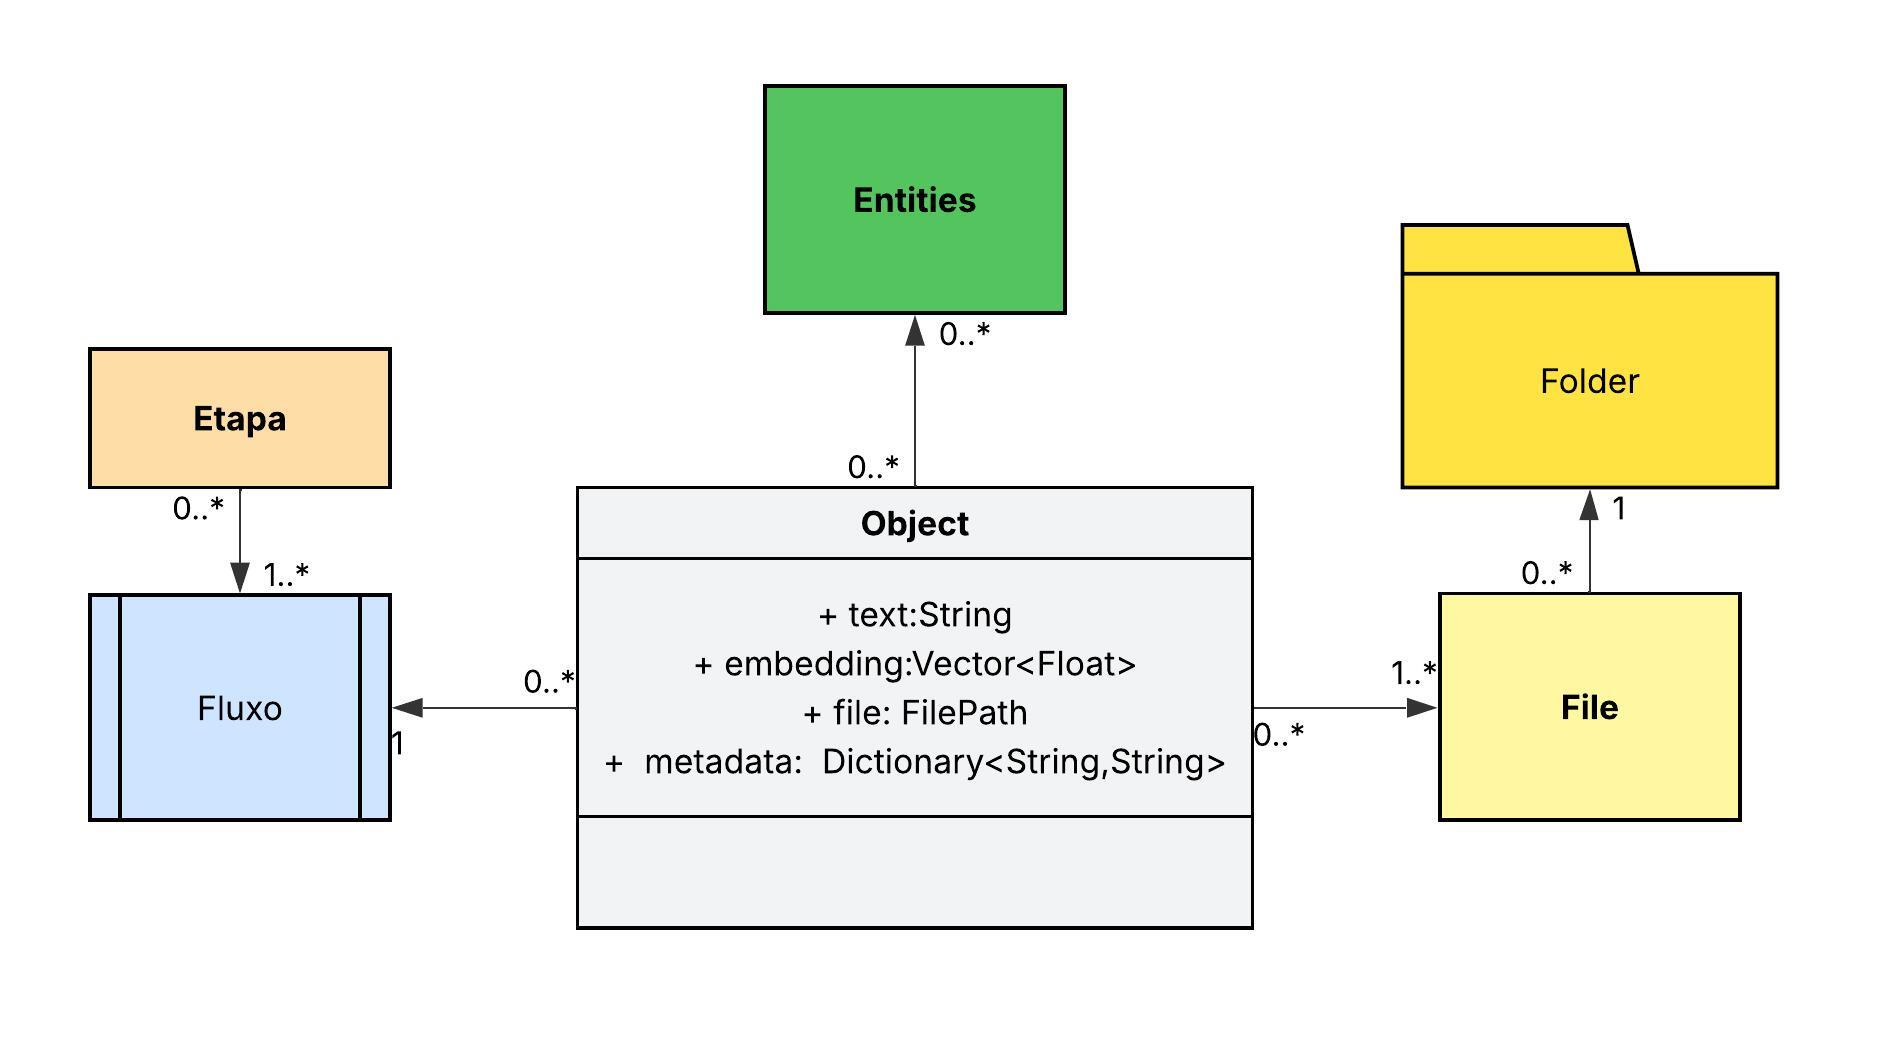
\includegraphics[width=1\linewidth]{Images/Classe UML.jpeg}
    \caption{Abstract UML representation of the schema structure, showing the relationships between objects, entities, folders, files, stages, and workflows in the Edoclink platform.}
    \label{fig:weaviate_class}
\end{figure}

As the research progressed, the schema was refined by embedding \textit{entities}, \textit{file paths}, and \textit{metadata} directly into the object representation. This ensured that objects became self-contained, enabling consistent deletion cascades and reducing reliance on cross-reference traversal for retrieval. The UML diagram in Figure~\ref{fig:weaviate_class} illustrates this abstract model, which was investigated as a candidate for efficient implementation. In practice, the real deployment within Edoclink is more complex, but this abstraction served as a foundation for evaluating design choices and guiding the development of scalable semantic retrieval. The results presented here should therefore be interpreted as a conceptual example rather than a one-to-one description of the production system.

Weaviate natively supports multiple collections in the same instance, and this functionality is employed in Edoclink to store independent datasets under a shared schema, with each instance exposed through web hooks. While not a methodological focus of this work, this results in a decentralized-like architecture, as data is distributed across multiple instances. This design increases the complexity of retrieval, since agents must identify and query the appropriate web hooks when traversing datasets.  

In summary, this section has focused on the database perspective: defining the schema, refining it through embedded fields, and placing it in the context of multi-tenant storage. The next section shifts attention to Agentic AI, where the challenge is not schema design but orchestrating retrieval with agents. This transition reflects the broader research landscape, where developments such as Weaviate’s Query Agent \cite{weaviate} exemplify the move toward automated reasoning layers capable of multi-step retrieval and problem solving.

\section{Weaviate MCP Server}

A \ac{MCP} \cite{mcp-architecture} server was developed to interface with a Weaviate vector database, with the primary goal of ensuring interoperability. This design enables clients such as \ac{LLM}-based agents to retrieve external information from Weaviate collections in a schema-aware manner. Since Weaviate databases typically enforce a strict schema, the server provides not only query tools but also memory of the available collections and their structure. This memory is extracted from the Weaviate schema endpoint and exposed to clients in
MCP resources, thereby contextualizing the agent with knowledge of valid properties, (function arguments to query a certain  before querying.  
The overall purpose of this server is to bridge structured information stored in Weaviate with powerful \ac{LLM} agents, using Anthropic’s standardized protocol for easier interoperability across different environments.

\subsection{Server Design}

The MCP server was implemented in Go and typescript, it was also implemented in Go because docker mcp-registry requires it for a pull request submission, also for it's easy reproducibility, and performance as a server because of it's concurrency capabilities. The docker mcp-registry is connected to docker. So if the pull request is accepted, MCP server will appear in official docker registry.

The server acts as an intermediary between clients and the Weaviate backend. It registers the necessary tools and resources to support both querying and schema inspection. By exposing schema information as MCP resources (e.g., \texttt{weaviate://schema/Dataset}), the server enables clients to discover the available collections and their properties (such as \texttt{targetProperties}: \{\texttt{text}: string, \texttt{filepath}: string\}). This ensures that all interactions with the database are schema-aware, preventing invalid queries.  

Clients are typically \ac{LLM}-powered agents capable of communicating over \ac{MCP}, which allows them to seamlessly integrate external structured knowledge into their reasoning processes.

\subsection{Functionality}
\begin{figure}[h]
    \centering
    \begin{tikzpicture}[node distance=2.2cm, >=latex, thick]

        % Nodes
        \node[draw, rounded corners, fill=blue!10, minimum width=4cm, minimum height=1cm, align=center] (client) {Client / LLM Agent};

        \node[draw, rounded corners, fill=green!10, minimum width=5cm, minimum height=1cm, below=of client, align=center] (mcp) {MCP Server \\ (Schema-aware middleware)};

        \node[draw, rounded corners, fill=orange!15, minimum width=5cm, minimum height=1cm, below=of mcp, align=center] (weaviate) {Weaviate Database \\ (Collections + Vectors)};

        % Arrows main flow
        \draw[->] (client) -- node[midway, right, text width=3.5cm, align=left] {Tool call (e.g. \texttt{weaviate-query})} (mcp);

        \draw[->] (mcp) -- node[midway, right, text width=3.8cm, align=left] {Validated request \\ (query + properties)} (weaviate);

        \draw[<-] (mcp) -- node[midway, left, text width=3.8cm, align=right] {Search results \\ (objects + properties)} (weaviate);

        \draw[<-] (client) -- node[midway, left, text width=3.5cm, align=right] {Structured MCP response \\ (ready for reasoning)} (mcp);

        % Schema discovery (dashed arrows)
        \draw[dashed, <->] (mcp.east) .. controls +(3,0) and +(3,0) .. (weaviate.east)
            node[midway, right, text width=4cm, align=center] {Schema discovery \\ (collections + fields \\ exposed as \\ \texttt{weaviate://schema/...})};

    \end{tikzpicture}
    \caption{Vertical system architecture of the MCP–Weaviate integration. The MCP server mediates queries, validates them against the Weaviate schema, and returns structured results to the client. Schema discovery is achieved dynamically through MCP resources.}
    \label{fig:system-architecture}
\end{figure}

